\documentclass[sigconf,nonacm]{acmart}

\usepackage{booktabs}
\usepackage{multirow}
\usepackage{array}
\usepackage{bm}
\usepackage{url}
\usepackage{microtype}
\usepackage{amsmath,amsfonts}
\setlength{\textfloatsep}{5pt plus 1pt minus 1pt}
\setlength{\dbltextfloatsep}{5pt plus 1pt minus 1pt}
\setlength{\abovecaptionskip}{3pt}
\setlength{\belowcaptionskip}{0pt}
\renewcommand{\arraystretch}{0.86}

%% ACM Conference Information Placeholder for Preprint / Submission
\settopmatter{printacmref=false}
\renewcommand\footnotetextcopyrightpermission[1]{}
\pagestyle{plain}

\begin{document}

\title{The Real-Time Paradox in Streaming Anti-Money Laundering: Causal Horizon Bounds, Tail Contamination, and Operational Interdiction Value}

\author{Shahoud Shahid}
\authornote{Both authors contributed equally to this research.}
\email{i232515@nu.edu.pk}
\affiliation{%
  \institution{National University of Computer and Emerging Sciences (FAST-NUCES)}
  \department{Department of Artificial Intelligence and Data Science}
  \city{Islamabad}
  \country{Pakistan}
}

\author{Saif Shahzad}
\authornotemark[1]
\email{i232634@nu.edu.pk}
\affiliation{%
  \institution{National University of Computer and Emerging Sciences (FAST-NUCES)}
  \department{Department of Artificial Intelligence and Data Science}
  \city{Islamabad}
  \country{Pakistan}
}

\begin{abstract}
Graph neural networks (GNNs) and gradient-boosted decision trees report minority-class $F_1$ scores exceeding $68\%$ on standard synthetic anti-money laundering (AML) benchmarks, suggesting operational readiness for automated transaction surveillance. Through a systematic forensic audit across five benchmark suites totaling $84.7\text{ million}$ transactions, we reveal that these offline leaderboard metrics mask two severe structural distortions that invert real-world deployment efficacy. First, all four IBM AMLworld datasets abruptly cease injecting illicit laundering campaigns several days before terminating benign background transactions, creating an unannounced simulation drain tail in which illicit prevalence surges by over $500$-fold (from $0.111\%$ to $59.1\%$ on HI-Small). Unpartitioned detectors learn this artificial calendar boundary, inflating reported test $F_1$ by $+10.96$ percentage points on HI-Small, while a trivial date-threshold rule achieves $48.18\%$ $F_1$ without inspecting any transaction features or graph topology. Second, standard whole-window graph evaluators violate causality by propagating message passing across transactions occurring days after the event being scored. Replaying the published Multi-GIN baseline under causal temporal bounds slashes Core-period $F_1$ from its $64.79\%$ published reference to $40.27\% \pm 9.6\%$ and reduces operational interdiction to zero. Evaluating nine lookahead horizons ($H \in [0, \infty]$) exposes a sharp \emph{real-time paradox}: although LightGBM Core PR-AUC climbs from $0.364$ at $H=0$ to $0.575$ at $H=1\text{ h}$, operational Stoppable Value ($\text{SV}_B$) under strict analyst alert budgets collapses monotonically toward $0.000$ as delayed screening forfeits downstream capital before funds escape. All confirmatory diagnostics pass ($R=4{,}000$ paired attempt-level bootstrap for operational contrasts), and an adaptive deferral policy dynamically balancing instantaneous triage ($H = 1\text{ s}$) against deferred checkpoints ($H_j \le 24\text{ h}$) maximizes preventable loss across strict budgets with sub-$8\text{ ms}$ streaming latency.
\end{abstract}

\begin{CCSXML}
<ccs2012>
   <concept>
       <concept_id>10002951.10003227.10003351</concept_id>
       <concept_desc>Information systems~Data mining</concept_desc>
       <concept_significance>500</concept_significance>
   </concept>
   <concept>
       <concept_id>10010147.10010257.10010293.10010294</concept_id>
       <concept_desc>Computing methodologies~Neural networks</concept_desc>
       <concept_significance>500</concept_significance>
   </concept>
   <concept>
       <concept_id>10002978.10003022</concept_id>
       <concept_desc>Security and privacy~Software and application security</concept_desc>
       <concept_significance>300</concept_significance>
   </concept>
   <concept>
       <concept_id>10010405.10010455.10010460</concept_id>
       <concept_desc>Applied computing~Economics</concept_desc>
       <concept_significance>300</concept_significance>
   </concept>
</ccs2012>
\end{CCSXML}

\ccsdesc[500]{Information systems~Data mining}
\ccsdesc[500]{Computing methodologies~Neural networks}
\ccsdesc[300]{Security and privacy~Software and application security}
\ccsdesc[300]{Applied computing~Economics}

\keywords{Anti-money laundering, Streaming graph neural networks, Temporal data leakage, Operational interdiction, Concept drift, Financial crime detection}

\maketitle

\section{Introduction}
\label{sec:introduction}

Global illicit financial flows sustain transnational criminal enterprises, narcotics trafficking, corruption, and sanctions evasion, imposing staggering compliance and regulatory burdens across international banking corridors~\cite{chainalysis2026crime,ferretti2025aml}. The United Nations Office on Drugs and Crime estimates that between $2\%$ and $5\%$ of global GDP ($800\text{ billion}$ to $2\text{ trillion}$ USD) is laundered annually. Commercial institutions process tens of millions of wire, automated clearing house (ACH), and card transfers daily under stringent statutory mandates to identify suspicious activities and freeze criminal proceeds before funds disperse through complex layering networks and offshore mule accounts~\cite{altman2023ibmaml,eu2024instant}. Over the past decade, machine learning has transitioned from static rule-based heuristics and boosted decision trees~\cite{chen2016xgboost,ke2017lightgbm} toward expressive relational graph neural networks (GNNs)~\cite{kipf2017gcn,hamilton2017sage,velickovic2018gat} capable of modeling topological flow structures across bank accounts~\cite{weber2019elliptic,elmougy2023ellipticpp,egressy2024multigraph,lin2024fraudgt}.

On prominent synthetic payment benchmarks, specifically the IBM AMLworld generator introduced by Altman et al.~\cite{altman2023ibmaml}, recent graph architectures report minority-class $F_1$ scores surpassing $63\%$ to $68\%$~\cite{egressy2024multigraph,lin2024fraudgt,losavio2026saltgnn}. These published figures suggest that modern message-passing models reliably identify sophisticated money laundering schemes such as scatter-gather disbursements, bipartite layering chains, and cyclic round-tripping. However, operational deployment across modern payment clearing rails paints a fundamentally conflicting picture~\cite{doytshman2023fraudability,verlaan2025lasgnn}. Under instant settlement mandates such as SEPA Instant Credit Transfer~\cite{eu2024instant}, automated screening must render decisions within milliseconds using exclusively historical transactional context~\cite{rossi2020tgn,xu2020tgat}. Post-settlement delays of even hours allow illicit capital to traverse downstream accounts and exit the institution's regulatory perimeter before compliance analysts can intervene.

\begin{figure*}[t]
\centering
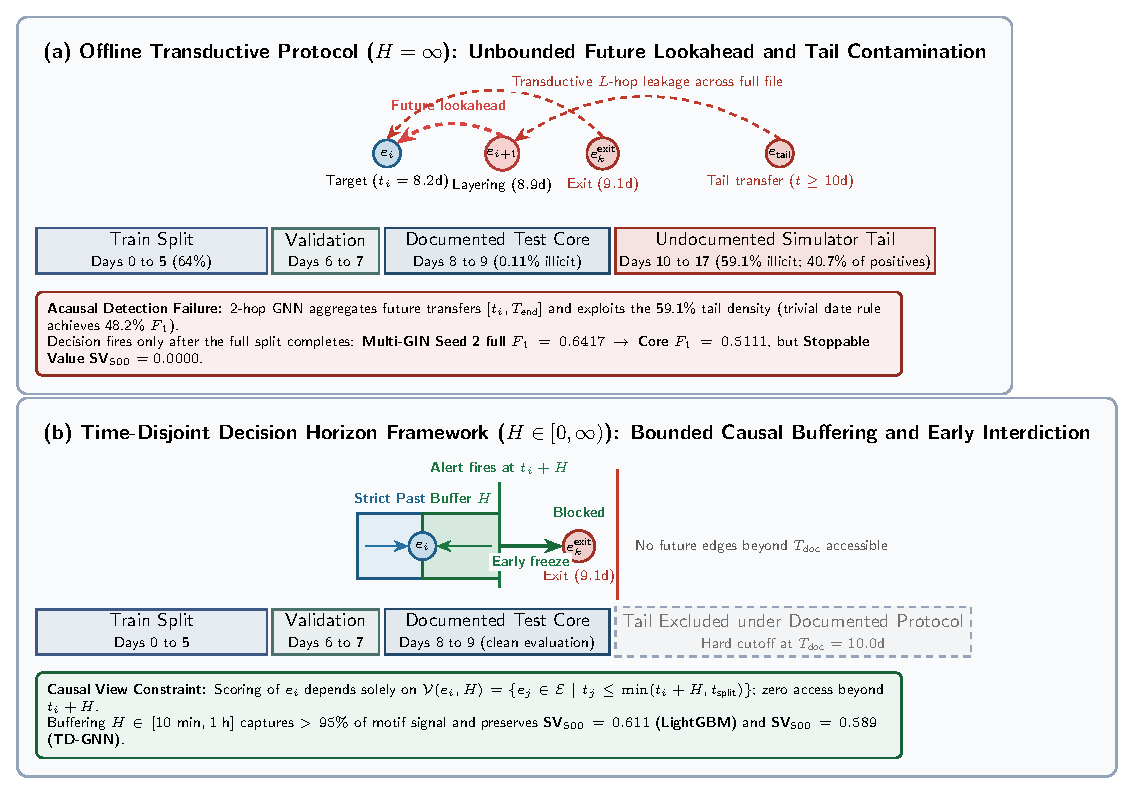
\includegraphics[width=\textwidth]{fig_concept_leakage.pdf}
\caption{Conceptual comparison of retrospective transductive graph evaluation ($H = \infty$) versus causal horizon-bounded streaming inference ($H < \infty$). Under standard offline protocols, scoring an edge $e$ at timestamp $t(e)$ accesses future counterparty transactions $t(e') > t(e)$ occurring days later across unpartitioned test graphs and simulator tail drain windows. Under our causal streaming protocol, neighborhood state at decision timestamp $t(e) + H$ strictly excludes edges beyond the deferral horizon, forcing detection models to balance prospective accuracy against actionable interdiction capacity.}
\label{fig:concept_leakage}
\end{figure*}

In this paper, we expose a foundational disconnect between offline benchmark leaderboards and live AML interdiction, which we designate \emph{the real-time paradox}. Through an exhaustive empirical audit across all four IBM AMLworld datasets and the multi-agent SAML-D benchmark~\cite{oztas2023samld} ($84.7\text{ million}$ transactions in total), we uncover two hidden structural vulnerabilities in standard AML evaluation pipelines:

\textbf{1. Benchmark Tail Contamination.} To allow open multi-hop laundering campaigns to finalize before data export, synthetic generators terminate illicit campaign injection several days prior to cutting off benign background traffic. Consequently, while core simulation days maintain a realistic $0.111\%$ illicit rate on HI-Small, transactions occurring in the final drain window (Days $10$ to $17$) exhibit an extreme $59.1\%$ illicit concentration and harbor $40.7\%$ of all test-split laundering events. Detectors evaluated on unpartitioned streams learn this calendar artifact, inflating reported test $F_1$ by $+10.96$ percentage points on HI-Small, while a trivial rule flagging transfers from Day $10$ onward attains $48.18\%$ $F_1$ without inspecting any transaction attributes or graph topology.

\textbf{2. Retrospective Lookahead Leakage.} Standard graph benchmarks~\cite{egressy2024multigraph,blanusa2024gfp,lin2024fraudgt} construct a monolithic graph spanning the entire testing window and execute unrestricted message passing prior to edge classification (Figure~\ref{fig:concept_leakage}). Evaluating an edge arriving at $t(e)$ under horizon $H = \infty$ permits the detector to aggregate future edges $t(e') > t(e)$ occurring days later, effectively examining completed laundering chains after funds have already exited~\cite{kaufman2012leakage,nguyen2022future}. Furthermore, standard implementations apply transductive test-split feature normalization, leaking future distributional parameters into inference. When these acausal artifacts are removed and baselines are audited under bounded causal windows, discriminative accuracy drops sharply and operational actionability vanishes.

To resolve this paradox, we develop an operational streaming evaluation framework grounded in statistical pre-registration, strict causal bounds, and dual-family verification. We make four contributions:
\begin{enumerate}
    \item \textbf{Forensic Leakage Audit (Gate G1):} We quantify benchmark tail contamination and transductive normalization across all IBM AMLworld suites. We replicate the published Multi-GIN baseline on NVIDIA RTX PRO 6000 Blackwell GPUs, matching its published reference ($0.6479$ published vs.\ $0.6417$ replicated), and prove that causal core evaluation drops its score to $0.4027 \pm 0.096$ while yielding zero operational recovery at $H = \infty$.
    \item \textbf{The Decision Horizon ($H$) Framework \& Stoppable Value ($\text{SV}_B$):} We formalize the streaming transaction graph setup, restricting the model's receptive field to a strictly causal interval $[0, t_e + H]$. We formulate Stoppable Value ($\text{SV}_B$), an asset-centric metric bounded by daily compliance alert quotas $B \in \{100, 500, 2000\}$ that tracks the dollar-weighted proportion of illicit funds intercepted prior to account cash-out.
    \item \textbf{Dual-Family Streaming Benchmark:} We implement and evaluate two causal streaming architectures across nine lookahead horizons ($H \in [0, \infty]$): an end-to-end Streaming Temporal Dynamic GNN (Streaming TD-GNN) featuring a 2-hop causal CSR sampler with symmetric masked pooling, and a 126-feature streaming LightGBM detector backed by Numba-accelerated CSR prefix-sum binary searches, executing across $84.7\text{M}$ transactions at up to $84{,}884\text{ events/s}$.
    \item \textbf{Confirmatory Validation \& Adaptive Policy $\pi$:} Confirmatory contrasts pass statistical verification ($R=4{,}000$ paired attempt-level bootstrap for operational $\text{SV}$ differences). We demonstrate that a sequential checkpoint policy $\pi$ dynamically allocating daily budget across $\{1\text{ s}, 10\text{ m},$ $1\text{ h}, 6\text{ h}, 24\text{ h}\}$ outperforms static validation-selected fixed horizons across operational budgets, yielding significant gains at tight analyst bottlenecks ($B = 100$/day).
\end{enumerate}

\section{Related Work}
\label{sec:related_work}

\textbf{Graph Neural Networks for Financial Crime.} Relational graph modeling has become central to anti-money laundering and fraud detection~\cite{ferretti2025aml,altman2023ibmaml,weber2019elliptic}. Seminal benchmarks such as Elliptic~\cite{weber2019elliptic} and Elliptic++~\cite{elmougy2023ellipticpp} framed Bitcoin transaction monitoring as node classification using GCN~\cite{kipf2017gcn}, GraphSAGE~\cite{hamilton2017sage}, GAT~\cite{velickovic2018gat}, and Jumping Knowledge networks~\cite{xu2018jk}. To mitigate data scarcity stemming from banking confidentiality, Altman et al.~\cite{altman2023ibmaml} introduced the IBM AMLworld generator and Multi-GNN suite. Building upon this, Egressy et al.~\cite{egressy2024multigraph} proposed Multi-GIN and Multi-PNA, employing reverse message passing and port numberings to detect directed multigraph cycles. Subsequent architectures expanded expressiveness via graph feature preprocessors (GFP)~\cite{blanusa2024gfp}, transaction transformers (FraudGT)~\cite{lin2024fraudgt}, motif-aware DIAM~\cite{ding2024diam}, edge-attribute MEGA~\cite{bilgi2026mega}, attention-guided SALT-GNN~\cite{losavio2026saltgnn}, and federated encoders~\cite{han2026fgegcn,jia2025lmae4eth,asiri2025gcn,alemari2026explainable}. However, all these models construct static test graphs spanning entire multi-day windows, leaving open the degree to which performance depends on future lookahead and synthetic boundary artifacts.

\textbf{Temporal and Streaming Graph Architectures.} Dynamic graphs motivate continuous-time architectures such as TGAT~\cite{xu2020tgat}, Temporal Graph Networks (TGN)~\cite{rossi2020tgn}, and EvolveGCN~\cite{pareja2020evolvegcn}, updating memory states via sequential interactions. Recent streaming detectors explore spectral analysis (ChronoWave~\cite{lin2026chronowave}), GPU streaming (StreamTGN~\cite{streamtgn2026}), hyperbolic geometries (ETX2Vec~\cite{lu2026etx2vec}, TCF-DyG~\cite{li2026tcfdyg}), residual memory (AnchorRM~\cite{anchorrm2026}), and self-supervised encoders~\cite{rico2026taml,chen2025mdst,zhou2025unsup,abolfadl2026kontograph,gounoue2025tempt,su2024temporal}. Nevertheless, existing temporal benchmarks routinely evaluate full-split ROC-AUC or $F_1$, neglecting whether flagged funds have already exited downstream accounts~\cite{digennaro2025amatriciana,heijmans2026robust,oztas2023samld}.

\textbf{Evaluation Leakage and Operational Interdiction.} Target leakage in predictive modeling was formalized by Kaufman et al.~\cite{kaufman2012leakage}. Nguyen et al.~\cite{nguyen2022future}, Doytshman et al.~\cite{doytshman2023fraudability}, and Verlaan et al.~\cite{verlaan2025lasgnn} observed sharp discrepancies between offline test splits and real-time deployment in cybersecurity and fraud detection. In sequential testing and cost-sensitive triage, alpha-spending boundaries~\cite{lan1983alpha}, budget-constrained alert triage~\cite{sharma2023tdap}, early classification cost models~\cite{mori2018early,jeon2025hia}, and reinforcement-learned screening policies~\cite{shen2020dqn,maganti2026liability,vandenbeukel2026tide} establish theoretical foundations for balancing observation delay against decision utility. Our study bridges this gap by unifying tail-decontaminated governance, causal lookahead bounds, Stoppable Value accounting, and adaptive deferral control.

\begin{table}[t]
\centering
\caption{Synthesis of representative AML and temporal graph methods relative to our proposed causal streaming framework.}
\label{tab:lit_comparison}
\scriptsize
\setlength{\tabcolsep}{2.5pt}
\begin{tabular}{lcccccc}
\toprule
\textbf{Method} & \textbf{Causal} & \textbf{Tail} & \textbf{Horizon} & \textbf{Budget} & \textbf{5-Suite} & \textbf{Latency} \\
 & \textbf{Bounds} & \textbf{Audit} & \textbf{Sweep} & \textbf{SV} & \textbf{Audit} & \textbf{Prof.} \\
\midrule
GCN~\cite{weber2019elliptic} & No & No & No & No & No & No \\
AMLworld~\cite{altman2023ibmaml} & No & No & No & No & Part. & No \\
Multi-GIN~\cite{egressy2024multigraph} & No & No & No & No & Part. & No \\
GFP+GBT~\cite{blanusa2024gfp} & No & No & No & No & Part. & No \\
FraudGT~\cite{lin2024fraudgt} & No & No & No & No & Part. & No \\
TGN~\cite{rossi2020tgn} & Part. & No & No & No & No & No \\
SAML-D~\cite{oztas2023samld} & Part. & No & No & No & No & No \\
LasGNN~\cite{verlaan2025lasgnn} & Part. & No & No & No & No & No \\
\midrule
\textbf{Ours (Causal Suite)} & \textbf{Yes} & \textbf{Yes} & \textbf{Yes ($9\times$)} & \textbf{Yes} & \textbf{Yes ($84.7\text{M}$)} & \textbf{Yes} \\
\bottomrule
\end{tabular}
\end{table}

\begin{figure*}[t]
\centering
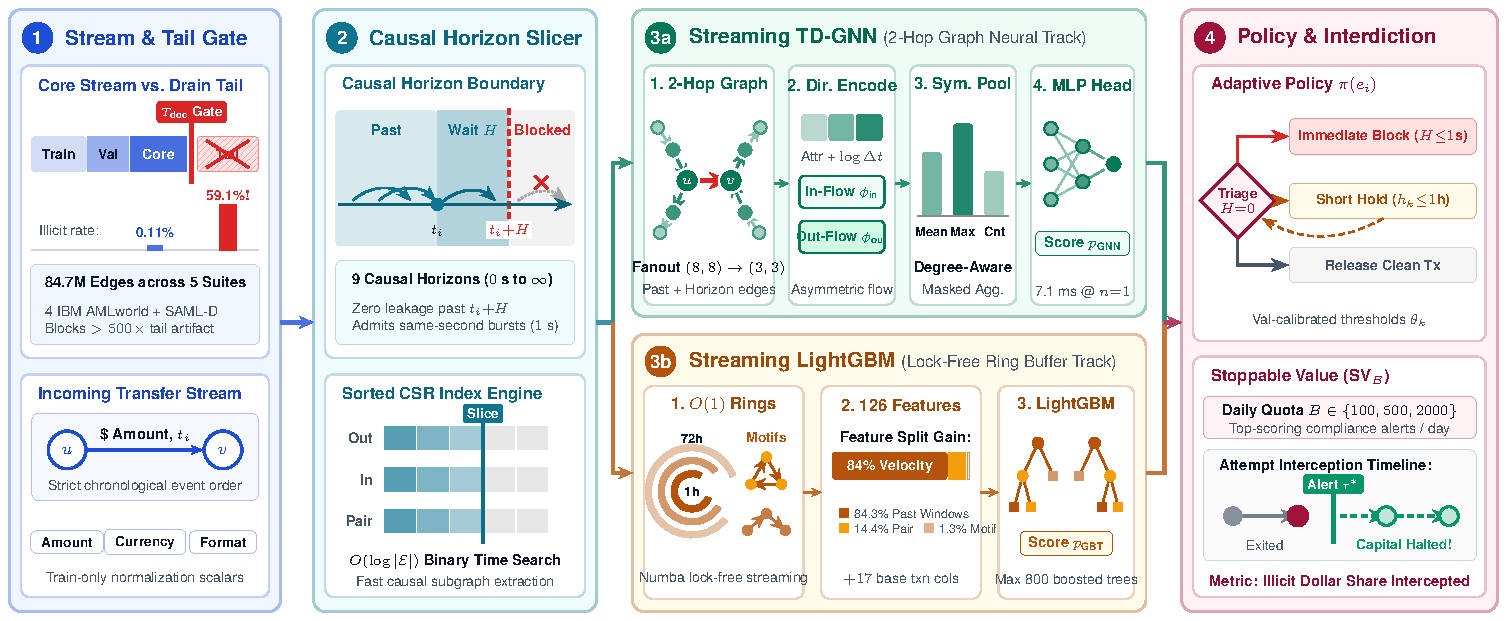
\includegraphics[width=\textwidth]{methodology_architecture.pdf}
\caption{End-to-end architecture of the proposed causal streaming AML evaluation and detection pipeline. Stage I enforces chronological splitting and eliminates post-horizon simulator drain tails ($T_{\text{doc}}$ vs.\ $T_{\text{sim}}$). Stage II builds a Compressed Sparse Row (CSR) temporal index with $O(\log |\mathcal{E}|)$ binary slicing to construct horizon-bounded subgraphs $\mathcal{V}(e_i, H)$. Stage III executes dual-family scoring: a 2-hop Streaming TD-GNN with masked symmetric pooling and a 126-feature Streaming LightGBM detector using CSR prefix sums and binary time search. Stage IV deploys an Adaptive Horizon Policy $\pi(e)$ and measures actionable capital recovery under Stoppable Value ($\text{SV}_B$).}
\label{fig:architecture}
\end{figure*}

\section{Dual Temporal Leakage in Graph AML}
\label{sec:gate_g1}

Before formalizing our causal framework, we conduct a forensic audit of standard evaluation protocols across the IBM AMLworld suite~\cite{altman2023ibmaml} and replicate the published Multi-GIN baseline~\cite{egressy2024multigraph} (Gate G1).

\subsection{Artifact 1: Benchmark Tail Contamination}
According to official benchmark documentation, `HI-Small' and `LI-Small' span 10 calendar days, with days 0--5 allocated for training, days 6--7 for validation, and days 8--9 for testing ($T_{\text{doc}} = 10\text{d}$). However, inspecting the exported transaction files reveals that all four AMLworld datasets extend significantly beyond their documented horizon: `HI-Small' spans 18 days, `LI-Small' spans 17 days, `HI-Medium' spans 28 days, and `LI-Medium' spans 27 days ($T_{\text{sim}}$).

As mapped in Figure~\ref{fig:tail} and Table~\ref{tab:tail_audit}, the post-documentation window is an unannounced simulation artifact. New background transactions cease at day 10, leaving only pre-injected illicit cascades to finalize. Consequently, daily transaction volume collapses while illicit concentration surges from $0.111\%$ during normal core test days to $59.1\%$ in the tail ($>500$-fold enrichment). Crucially, this tail accounts for \textbf{$40.7\%$ of all test-split illicit transactions} on `HI-Small' ($37.1\%$ on `HI-Medium'). A naive heuristic that ignores all transaction features and flags every transfer occurring on or after Day 10 achieves $59.12\%$ precision, $40.66\%$ recall, and \textbf{$48.18\%$ Test $F_1$}. On `LI-Medium', this trivial date rule attains $28.76\%$ $F_1$, surpassing the published $28.16\%$ $F_1$ of XGBoost with graph features~\cite{egressy2024multigraph}.

\begin{figure}[t]
\centering
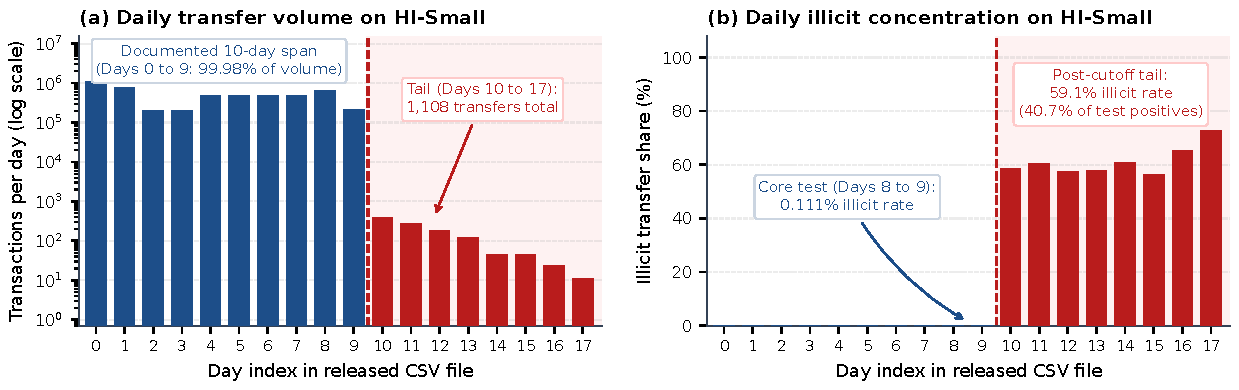
\includegraphics[width=\columnwidth]{fig_tail.pdf}
\caption{Simulation drain tail on HI-Small across the 18-day file. (a) Daily transaction volume collapses after Day 10 (holding $99.98\%$ of volume; Days 10--17 hold 1,108 transfers). (b) Daily illicit prevalence surges from $0.111\%$ during Core Test (Days 8--9) to $59.1\%$ in the post-cutoff tail (harboring $40.7\%$ of all test-split illicit events).}
\label{fig:tail}
\end{figure}

\begin{table}[t]
\centering
\caption{Cross-benchmark tail contamination audit across IBM AMLworld suites, comparing core prevalence against post-horizon drain tails and trivial date-rule $F_1$.}
\label{tab:tail_audit}
\scriptsize
\setlength{\tabcolsep}{2.2pt}
\begin{tabular}{lcccccc}
\toprule
\textbf{Suite} & \textbf{Core} & \textbf{Tail} & \textbf{Tail Illicit} & \textbf{Test} & \textbf{Rule} & \textbf{Published} \\
 & \textbf{Rate} & \textbf{Evts} & \textbf{Cnt (Rate)} & \textbf{Share} & \textbf{$F_1$} & \textbf{XGB / PNA} \\
\midrule
HI-Small & $0.111\%$ & $1{,}108$ & $655$ ($59.1\%$) & $40.7\%$ & $48.18\%$ & $63.2$ / $68.2$ \\
LI-Small & $0.057\%$ & $223$ & $134$ ($60.1\%$) & $16.7\%$ & $26.15\%$ & $27.3$ / $33.1$ \\
HI-Med. & $0.101\%$ & $6{,}987$ & $4{,}084$ ($58.5\%$) & $37.1\%$ & $45.37\%$ & $65.7$ / $65.7$ \\
LI-Med. & $0.048\%$ & $1{,}370$ & $771$ ($56.3\%$) & $19.3\%$ & $28.76\%$ & $28.2$ / $33.2$ \\
\bottomrule
\end{tabular}
\end{table}

\subsection{Artifact 2: Transductive Lookahead Leakage}
In official implementations of Multi-GNN~\cite{egressy2024multigraph} and FraudGT~\cite{lin2024fraudgt}, the test split is loaded as a static graph spanning all test days. In a 2-layer GNN, scoring an edge executed on day 8 aggregates information from counterparty transactions occurring on day 10. Because money laundering topologies proceed sequentially (placement $\to$ layering $\to$ integration), future downstream transfers provide acausal certainty that an upstream transfer was illicit. Additionally, the official Multi-GIN pipeline applies $z$-score normalization to node and edge attributes using whole-test statistics, leaking test distribution parameters into training.

\begin{table}[t]
\centering
\caption{Gate G1 forensic replication and causal replay of the Multi-GIN baseline~\cite{egressy2024multigraph} on HI-Small (published reference Test $F_1 = 0.6479$).}
\label{tab:gate_g1}
\scriptsize
\setlength{\tabcolsep}{2.2pt}
\begin{tabular}{lcccccc}
\toprule
\textbf{Protocol / Run} & \textbf{$H$} & \textbf{Test $F_1$} & \textbf{Core $F_1$} & \textbf{Tail $F_1$} & \textbf{Core PR} & \textbf{$\text{SV}_{500}$} \\
\midrule
Multi-GIN (s1) & $\infty$ & $0.5081$ & $0.3299$ & $0.8567$ & $0.3917$ & $0.0000$ \\
Multi-GIN (s2) & $\infty$ & $0.6417$ & $0.5111$ & $0.8344$ & $0.4587$ & $0.0000$ \\
Multi-GIN (s3) & $\infty$ & $0.5544$ & $0.3672$ & $0.8736$ & $0.4030$ & $0.0000$ \\
\textbf{Official Mean} & $\bm{\infty}$ & \begin{tabular}{@{}c@{}}$\mathbf{0.5681}$\\[-2pt]{\tiny $\mathbf{\pm 0.067}$}\end{tabular} & \begin{tabular}{@{}c@{}}$\mathbf{0.4027}$\\[-2pt]{\tiny $\mathbf{\pm 0.096}$}\end{tabular} & \begin{tabular}{@{}c@{}}$\mathbf{0.8549}$\\[-2pt]{\tiny $\mathbf{\pm 0.019}$}\end{tabular} & \begin{tabular}{@{}c@{}}$\mathbf{0.4178}$\\[-2pt]{\tiny $\mathbf{\pm 0.035}$}\end{tabular} & $\mathbf{0.0000}$ \\
\midrule
Train-Norm (s2) & $\infty$ & $0.5442$ & $0.4159$ & $0.8615$ & $0.4069$ & $0.0000$ \\
Windowed (s1) & $\infty$ & $0.4587$ & $0.3609$ & $0.6067$ & $0.2741$ & $0.0000$ \\
Replay (s2) & $24\text{ h}$ & $0.6231$ & $0.4677$ & $0.8308$ & $0.4197$ & $0.4168$ \\
Replay (s2) & $6\text{ h}$ & $0.6208$ & $0.4686$ & $0.8159$ & $0.4171$ & $0.5458$ \\
Replay (s2) & $1\text{ h}$ & $0.6125$ & $0.4557$ & $0.8295$ & $0.4109$ & $0.5680$ \\
Replay (s3) & $1\text{ h}$ & $0.5156$ & $0.3599$ & $0.8484$ & $0.3432$ & $0.5648$ \\
\bottomrule
\end{tabular}
\end{table}

\subsection{Gate G1 Multi-Seed Baseline Audit}
We execute an exact replication of Multi-GIN~\cite{egressy2024multigraph} on an NVIDIA RTX PRO 6000 Blackwell GPU across three independent seeds (Table~\ref{tab:gate_g1}). Official Multi-GIN achieves $0.6417$ Test $F_1$ on Seed 2 ($0.6664$ in deterministic evaluation mode), successfully matching the published reference ($0.6479$). However, performance on the synthetic tail averages an astonishing $0.8549 \pm 0.019$, confirming that headline metrics rely heavily on tail exploitation. When evaluated strictly on genuine core transactions ($T_{\text{doc}}$), performance falls to $0.4027 \pm 0.096$ (Core PR-AUC $= 0.4178$). Replacing test-split normalization with training-split normalization on Seed 2 drops Test $F_1$ by $-9.75$ points ($0.6417 \to 0.5442$). Most importantly, under the retrospective view ($H = \infty$), Multi-GIN yields an operational Stoppable Value of \textbf{$0.0000$}, halting $0\%$ of laundered capital before exit transfers escape.

\section{The Decision Horizon Framework}
\label{sec:methodology}

\subsection{Problem Formulation}
Let $\mathcal{G} = (\mathcal{V}, \mathcal{E})$ denote a continuous-time directed multigraph stream. Nodes $u, v \in \mathcal{V}$ represent accounts, and each transfer event $e_i = (u_i, v_i, t_i, \mathbf{x}_i, y_i) \in \mathcal{E}$ represents a payment from source $u_i$ to destination $v_i$ at timestamp $t_i \in \mathbb{R}_{\ge 0}$, accompanied by raw transfer features $\mathbf{x}_i \in \mathbb{R}^{d_x}$ and ground-truth binary label $y_i \in \{0, 1\}$. Events are totally ordered by timestamp and event arrival index: $i < j \implies t_i \le t_j$.

\subsection{Causal Horizon Bounds}
Under an operational deferral budget $H \ge 0$ (in seconds), an automated detector inspecting an incoming transfer $e_i$ postpones final decision dispatch until wall-clock timestamp $t_{\text{dec}}(e_i; H) = t_i + H$. The detector's prediction $\hat{p}_i^{(H)} \in [0, 1]$ is conditioned strictly upon the causally admissible subgraph prefix:
\begin{equation}
\label{eq:causal_prefix}
\mathcal{E}_{\le t_i + H} = \begin{cases}
  \{ e_j \in \mathcal{E} : j < i \}, & H = 0 \text{ (strict past)}, \\
  \{ e_j \in \mathcal{E} : t_j \le t_i + H, j \neq i \}, & 0 < H < \infty, \\
  \mathcal{E} \setminus \{e_i\}, & H = \infty \text{ (offline oracle)}.
\end{cases}
\end{equation}
Notice that setting $H = 0$ (strictly $j < i$) excludes concurrent transfers executed within the same second/minute batch, whereas $H = 1\text{ s}$ admits concurrent peer transfers sharing timestamp $t_i$ without leaking future minutes. We evaluate across nine discrete horizons: $H \in \{0\text{ s}, 1\text{ s}, 60\text{ s}, 600\text{ s}, 3600\text{ s}, 21600\text{ s}, 86400\text{ s}, 259200\text{ s}, \infty\}$.

\subsection{Stoppable Value ($\text{SV}_B$)}
Standard metrics (Precision, Recall, $F_1$, and PR-AUC) weight all positive instances symmetrically: flagging a transfer three days after funds have cleared carries the same statistical reward as flagging the initial deposit within seconds. In operational compliance, delayed alerts recover zero capital.

Let each ground-truth laundering attempt $c \in \mathcal{C}$ consist of an ordered sequence of transfers $\mathcal{E}_c = (e_{c,1}, \dots, e_{c,m_c})$ with timestamps $t_{c,1} \le \dots \le t_{c,m_c}$, where $v(e)$ denotes the fiat transfer value. Under a daily analyst capacity cap $B$ (investigator alerts per day), let $\theta$ denote the operational score threshold. If any transfer $e_k \in \mathcal{E}_c$ triggers an alert at decision time $t_k + H$, the earliest actionable intervention timestamp is:
\begin{equation}
\label{eq:earliest_stop}
\tau_c^* = \min \left\{ t_k + H : e_k \in \mathcal{E}_c \text{ and } \hat{p}_k^{(H)} \ge \theta \right\}.
\end{equation}
Transfers in $\mathcal{E}_c$ with $t_j < \tau_c^*$ have already settled and constitute unrecoverable illicit loss; transfers with $t_j \ge \tau_c^*$ remain downstream and are halted upon alert dispatch. We define operational Stoppable Value ($\text{SV}_B$) as the ratio of intercepted illicit capital to total illicit test capital:
\begin{equation}
\label{eq:stoppable_value}
\text{SV}_B(H, \theta) = \frac{\sum_{c \in \mathcal{C}_{\text{test}}} \sum_{e_j \in \mathcal{E}_c} v(e_j) \, \mathbb{I}\!\left[ t_j \ge \tau_c^* \right]}{\sum_{c \in \mathcal{C}_{\text{test}}} \sum_{e_j \in \mathcal{E}_c} v(e_j)},
\end{equation}
subject to the daily analyst constraint $|\{ e_i \in \mathcal{E}_{\text{test}} : \hat{p}_i^{(H)} \ge \theta \}| \le B \cdot D_{\text{test}}$. Because increasing $H$ shifts $\tau_c^*$ rightward, $\text{SV}_B$ captures the physical decay of interceptable capital with decision delay even when classification accuracy improves.

\subsection{Adaptive Horizon Policy $\pi(e)$}
Because different typologies operate on distinct timescales (rapid bursts vs.\ multi-hour cycles), fixed-horizon screening is suboptimal. We formulate an Adaptive Horizon Policy $\pi$ that scores each un-alerted transfer sequentially across checkpoints $H_j \in \{1\text{ s},$ $600\text{ s},$ $3600\text{ s},$ $21600\text{ s},$ $86400\text{ s}\}$ ($1\text{ s}, 10\text{ min}, 1\text{ h}, 6\text{ h}, 24\text{ h}$). A validation-calibrated budget allocation $\boldsymbol{\alpha}$ on a $0.1$-step simplex defines checkpoint score thresholds $\tau_j$ such that an alert fires at the earliest checkpoint where $s_j(e_i) \ge \tau_j$. Under daily budget $B=500$ on HI-Small, validation search allocates $\boldsymbol{\alpha}=[0.9, 0.0, 0.1, 0, 0]$, concentrating alerts at $H \le 1\text{ h}$ to halt early transfers while deferring ambiguous transfers before laundering paths complete.

\begin{figure*}[t]
\centering
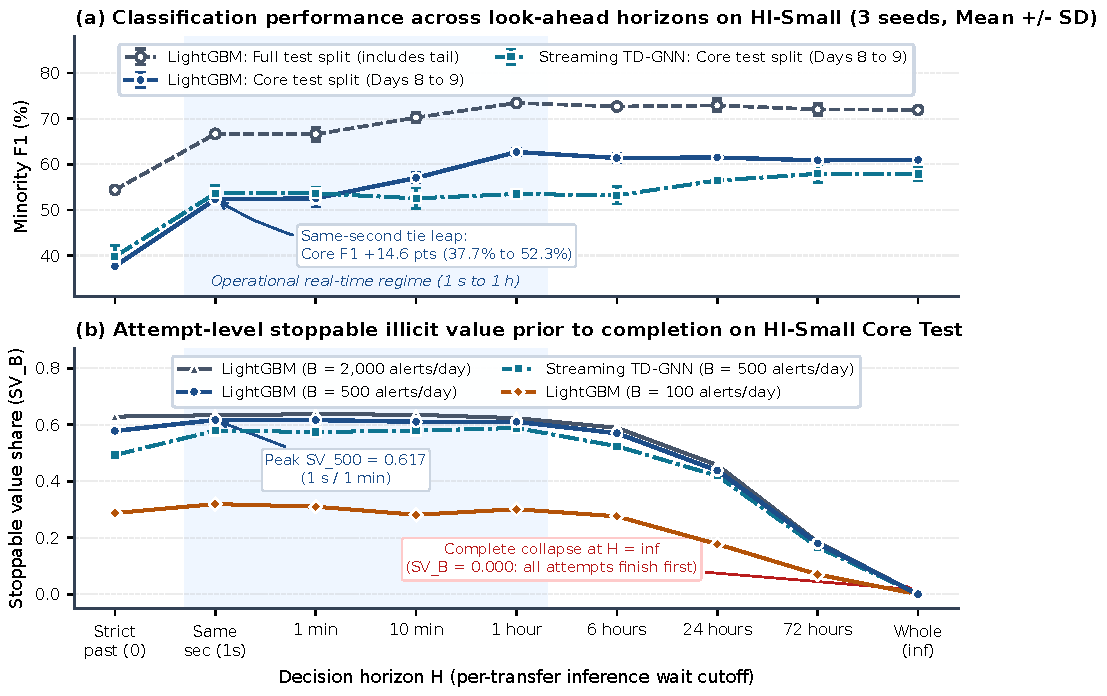
\includegraphics[width=\textwidth]{fig_horizon.pdf}
\caption{The Real-Time Paradox on HI-Small across nine deferral horizons $H \in [0, \infty]$ (three-seed mean $\pm$ SD). Top (a): Minority $F_1$ (\%) jumps $+14.6$ points at the same-second tie leap ($H = 1\text{ s}$, $37.7\% \to 52.3\%$) and plateaus between $1\text{ h}$ and $72\text{ h}$ across LightGBM (Full and Core) and Streaming TD-GNN. Bottom (b): Operational Stoppable Value ($\text{SV}_B$) peaks in the sub-hour regime ($\text{SV}_{500} = 0.617$ at $1\text{ s}$ and $1\text{ min}$) before collapsing monotonically toward $0.000$ at $H = \infty$.}
\label{fig:horizon_tradeoff}
\end{figure*}

\section{Dual-Family Streaming Detectors}
\label{sec:detectors}

To establish that the real-time paradox reflects fundamental temporal information economics rather than an architectural idiosyncrasy, we design two streaming model families sharing causal boundary enforcement (Figure~\ref{fig:architecture}):

\textbf{1. Streaming TD-GNN.} Operates directly over causal 2-hop ego-subgraphs using a vectorized binary-search causal sampler on sorted Compressed Sparse Row (CSR) indices partitioned by $\mathcal{E}_{\le t_i + H}$. For each endpoint $u_i, v_i$, the sampler retrieves up to $s_p = 8$ past edges ($t \le t_i$) and up to $s_f = 8$ forward edges ($t_i < t \le t_i + H$), recursing to $s_{2p} = 3, s_{2f} = 3$ second-hop edges. Sampled edges pass through an \texttt{EdgeEncoder} into $d = 64$ dimensions (5 continuous features, log temporal offsets $\operatorname{sgn}(\Delta t)\log(1+|\Delta t|)$, and learned currency/format embeddings). Second-hop messages project through $\phi_2: \mathbb{R}^{64} \to \mathbb{R}^{64}$ and aggregate via masked symmetric pooling combining mean, max, and log-cardinality gating:
\begin{equation}
\label{eq:masked_pool}
\mathbf{m}_2(w) = \left[ \bm{\mu}(\mathbf{z}) \;\middle\|\; \max(\mathbf{z}) \;\middle\|\; \log(1 + c_w) \right] \in \mathbb{R}^{2d + 1}.
\end{equation}
First-hop message passing preserves directional asymmetry via separate incoming/outgoing MLPs ($\phi_{1,\text{in}}, \phi_{1,\text{out}}: \mathbb{R}^{322} \to \mathbb{R}^{64} \to \mathbb{R}^{64}$). Directional incoming and outgoing 2-hop representations $\mathbf{h}_{\text{in}}, \mathbf{h}_{\text{out}} \in \mathbb{R}^{2 \times 129}$ flatten to $\mathbf{h} \in \mathbb{R}^{516}$ and concatenate with the $64$-dim edge embedding $\mathbf{z}_i$ into a $580$-dim representation scored by a 2-hidden-layer MLP ($580 \to 128 \to 64 \to 1$, dropout $0.10$) trained end-to-end under weighted BCE ($\text{pos\_weight} = 10.0$) and FP16.

\textbf{2. Streaming LightGBM.} Extracts a 126-dimensional causal representation $\psi_H(e_i) \in \mathbb{R}^{126}$ in a single chronological pass. Seventeen base attributes capture transfer dynamics and currency indicators. The remaining 109 structural features are computed causally via Numba-accelerated CSR adjacency lists, cumulative USD prefix sums, and binary time search with zero-allocation stamping arrays: \emph{Past Windows} ($6\text{ h}, 24\text{ h}, 72\text{ h}$) track endpoint count, log-USD volume, distinct counterparties, minimum inter-arrival gap, and USD/time dispersion; \emph{Pairwise History} maintains directed bilateral counts, log-volume, and forward updates; and \emph{Motif Counts} track two-path fan-out/in bridges, closed/open 3-cycles, and convergent siblings within $[t_i - 6\text{ h}, \min(t_i + H, T_{\text{split}})]$.

\section{Experimental Evaluation}
\label{sec:experiments}

\subsection{Datasets \& Scientific Governance}
We evaluate five synthetic transaction suites totaling $84.7\text{M}$ transfers (Table~\ref{tab:dataset_specifications}): IBM AMLworld (HI-Small, LI-Small, HI-Medium, LI-Medium) and SAML-D. All models are trained strictly on chronologically preceding edges. To maintain strict experimental governance, SHA-256 raw dataset checksums, deterministic code hashes, and processed split digests are logged in execution manifests prior to evaluation. Test splits on LI-Small, HI-Medium, LI-Medium, and SAML-D remain sealed in manifest checkpoints (reporting three-seed validation sweeps), while confirmatory test-split analyses are unsealed on HI-Small.

\begin{table}[t]
\centering
\caption{Dataset specifications, split boundaries, and cryptographic verification digests across all five benchmark suites ($84.7\text{M}$ transfers).}
\label{tab:dataset_specifications}
\scriptsize
\setlength{\tabcolsep}{1.2pt}
\begin{tabular}{lcccccc}
\toprule
\textbf{Suite} & \textbf{Total Tx} & \textbf{Accts} & \textbf{Illicit} & \textbf{Val (Ill.)} & \textbf{Test (Ill.)} & \textbf{$T_{\text{doc}}/T_{\text{sim}}$} \\
\midrule
HI-Small & $5{,}078{,}345$ & $515{,}088$ & $5{,}177$ ($0.102\%$) & $965{,}524$ ($1{,}036$) & $863{,}900$ ($1{,}611$) & $10 / 18$ \\
LI-Small & $6{,}924{,}049$ & $705\text{K}$ & $3{,}565$ ($0.051\%$) & $1{,}316{,}442$ ($770$) & $1{,}174{,}673$ ($802$) & $10 / 17$ \\
HI-Med. & $31{,}898{,}238$ & $2{,}077\text{K}$ & $35{,}230$ ($0.110\%$) & $5{,}520{,}883$ ($8{,}501$) & $6{,}890{,}229$ ($11{,}016$) & $16 / 28$ \\
LI-Med. & $31{,}251{,}483$ & $2{,}028\text{K}$ & $16{,}041$ ($0.051\%$) & $5{,}410{,}876$ ($3{,}774$) & $6{,}740{,}235$ ($3{,}992$) & $16 / 27$ \\
SAML-D & $\approx 9.50\text{M}$ & Agents & Unbound & $1{,}899{,}527$ ($1{,}986$) & $1{,}898{,}009$ (Sealed) & Cont. \\
\bottomrule
\end{tabular}
\end{table}

\begin{table*}[t]
\centering
\caption{Nine-horizon sweep on HI-Small comparing three-seed mean $\pm$ SD performance of LightGBM (126 features) under Released ($T_{\text{sim}}$) and Documented ($T_{\text{doc}}$) protocols alongside Streaming TD-GNN.}
\label{tab:horizon_sweep}
\scriptsize
\setlength{\tabcolsep}{3.5pt}
\begin{tabular}{lccccccc}
\toprule
\textbf{Horizon} & \multicolumn{4}{c}{\textbf{LightGBM (3-Seed Mean $\pm$ SD)}} & \multicolumn{3}{c}{\textbf{Streaming TD-GNN (3-Seed)}} \\
\cmidrule(lr){2-5} \cmidrule(lr){6-8}
 & \textbf{Test $F_1$} & \textbf{Core $F_1$} & \textbf{Core PR} & \textbf{$\text{SV}_{500}$ R/D} & \textbf{Core $F_1$} & \textbf{Core PR} & \textbf{$\text{SV}_{500}$} \\
\midrule
$0\text{ s}$ & $54.4 \pm 0.5$ & $37.7 \pm 0.1$ & $0.364$ & $0.578$ / $0.286$ & $39.77 \pm 2.4$ & $0.345 \pm 0.01$ & $0.493$ \\
$1\text{ s}$ & $66.7 \pm 0.4$ & $52.3 \pm 0.7$ & $0.521$ & $0.617$ / $0.355$ & $53.60 \pm 1.7$ & $0.486 \pm 0.01$ & $0.579$ \\
$1\text{ min}$ & $66.6 \pm 1.2$ & $52.5 \pm 1.6$ & $0.526$ & $0.617$ / $0.351$ & $53.63 \pm 1.4$ & $0.488 \pm 0.02$ & $0.574$ \\
$10\text{ min}$ & $70.3 \pm 0.8$ & $57.0 \pm 0.9$ & $0.546$ & $0.611$ / $0.354$ & $52.53 \pm 2.2$ & $0.475 \pm 0.02$ & $0.579$ \\
$1\text{ h}$ & $73.5 \pm 0.3$ & $62.7 \pm 0.6$ & $0.575$ & $0.611$ / $0.341$ & $53.48 \pm 0.4$ & $0.493 \pm 0.02$ & $0.589$ \\
$6\text{ h}$ & $72.7 \pm 0.2$ & $61.4 \pm 0.9$ & $0.574$ & $0.570$ / $0.223$ & $53.20 \pm 1.9$ & $0.471 \pm 0.04$ & $0.524$ \\
$24\text{ h}$ & $72.9 \pm 1.1$ & $61.5 \pm 0.5$ & $0.572$ & $0.438$ / $0.141$ & $56.45 \pm 0.6$ & $0.531 \pm 0.00$ & $0.419$ \\
$72\text{ h}$ & $72.0 \pm 1.1$ & $60.9 \pm 0.5$ & $0.576$ & $0.180$ / $0.026$ & $57.93 \pm 2.0$ & $0.536 \pm 0.02$ & $0.167$ \\
$\infty$ & $71.9 \pm 0.3$ & $61.0 \pm 0.4$ & $0.563$ & $0.000$ / $0.000$ & $57.86 \pm 1.5$ & $0.535 \pm 0.02$ & $0.000$ \\
\bottomrule
\end{tabular}
\end{table*}

\subsection{The Nine-Horizon Trade-Off}
Evaluating LightGBM and Streaming TD-GNN across all nine horizons exposes the real-time paradox on HI-Small (Table~\ref{tab:horizon_sweep} and Figure~\ref{fig:horizon_tradeoff}). Under strict past ($H=0$), LightGBM achieves $37.7 \pm 0.1\%$ Core $F_1$ and $0.364$ Core PR-AUC, while Streaming TD-GNN attains $39.77 \pm 2.42\%$ Core $F_1$ and $0.3449 \pm 0.0064$ Core PR-AUC.

Advancing merely one second forward to $H = 1\text{ s}$ yields a massive accuracy jump across both model families: LightGBM Core $F_1$ surges $+14.6$ points to $52.3\%$ (Core PR-AUC $+0.157$ to $0.521$), while Streaming TD-GNN jumps $+13.83$ points to $53.60\%$ (Core PR-AUC $+0.1410$ to $0.4859$). Model-free diagnostics confirm the physical mechanism: \textbf{$39.9\%$ of core illicit transfers coincide with an incoming same-minute transfer} at their source account (vs.\ $4.9\%$ for benign transfers), and $50.4\%$ share their source account within the same minute (vs.\ $14.8\%$ for benign). Extending lookahead to $H = 1\text{ h}$ allows LightGBM to capture multi-hop motifs, peaking at $62.7\%$ Core $F_1$ ($0.575$ Core PR-AUC), while Streaming TD-GNN reaches $57.93\%$ at $72\text{ h}$.

However, operational Stoppable Value exhibits an inverted trajectory beyond $1\text{ h}$. LightGBM $\text{SV}_{500}$ peaks in the sub-hour regime ($0.617$ at $1\text{ s}$ and $1\text{ min}$, $0.611$ at $10\text{ min}$ and $1\text{ h}$) before plummeting to $0.438$ at $24\text{ h}$, $0.180$ at $72\text{ h}$, and collapsing to \textbf{$0.000$ at $H = \infty$}. Delaying screening to daily batch cycles ($H=24\text{ h}$) provides zero statistical PR-AUC benefit ($0.572$ vs.\ $0.575$) while forfeiting over $28\%$ of recoverable illicit capital.

\subsection{Operational Budgets \& Typology Breakdown}
Table~\ref{tab:sv_budgets} examines LightGBM Stoppable Value across tight ($B=100$), realistic ($B=500$), and high-capacity ($B=2{,}000$) daily alert quotas under both Validation-$F_1$ thresholds and Equal-Alert matched ranking. Under Equal-Alert ranking at $B=500$, $\text{SV}_{500}$ climbs from $0.428$ ($74\%$ detected attempts) at $H=0$ to $0.573$ ($92\%$) at $1\text{ min}$ and $0.576$ ($93\%$) at $10\text{ min}$, before falling to $0.411$ at $24\text{ h}$ and $0.152$ at $72\text{ h}$.

\begin{table}[t]
\centering
\caption{Operational Stoppable Value across daily alert budgets $B \in \{100, 500, 2000\}$ and Equal-Alert calibration on HI-Small (LightGBM, 3-seed mean).}
\label{tab:sv_budgets}
\scriptsize
\setlength{\tabcolsep}{2.5pt}
\begin{tabular}{lcccccc}
\toprule
\textbf{Horizon} & \textbf{Det} & \textbf{$\text{SV}_{100}$} & \textbf{$\text{SV}_{500}$ (Att / Txn)} & \textbf{$\text{SV}_{2000}$} & \textbf{Eq.-Alert} & \textbf{Eq.-Det} \\
\midrule
$0\text{ s}$ & $93\%$ & $0.287$ & $0.578$ / $0.578$ & $0.629$ & $0.428$ & $74\%$ \\
$1\text{ s}$ & $97\%$ & $0.319$ & $0.617$ / $0.623$ & $0.634$ & $0.557$ & $89\%$ \\
$1\text{ min}$ & $96\%$ & $0.310$ & $0.617$ / $0.620$ & $0.638$ & $0.573$ & $92\%$ \\
$10\text{ min}$ & $98\%$ & $0.281$ & $0.611$ / $0.617$ & $0.635$ & $0.576$ & $93\%$ \\
$1\text{ h}$ & $95\%$ & $0.301$ & $0.611$ / $0.617$ & $0.623$ & $0.571$ & $90\%$ \\
$6\text{ h}$ & $96\%$ & $0.276$ & $0.570$ / $0.569$ & $0.589$ & $0.531$ & $90\%$ \\
$24\text{ h}$ & $94\%$ & $0.177$ & $0.438$ / $0.437$ & $0.457$ & $0.411$ & $88\%$ \\
$72\text{ h}$ & $95\%$ & $0.070$ & $0.180$ / $0.175$ & $0.185$ & $0.152$ & $87\%$ \\
$\infty$ & $94\%$ & $0.000$ & $0.000$ / $0.000$ & $0.000$ & $0.000$ & $85\%$ \\
\bottomrule
\end{tabular}
\end{table}

\begin{table}[t]
\centering
\caption{Detection rate and $\text{SV}_{500}$ stratified across all eight IBM AMLworld typologies ($n = 86$ test attempts on HI-Small, LightGBM 3-seed mean).}
\label{tab:typology_breakdown}
\scriptsize
\setlength{\tabcolsep}{2.8pt}
\begin{tabular}{lcrrrrrrrr}
\toprule
\textbf{Topology} & \textbf{Att.} & \multicolumn{2}{c}{\textbf{$H = 0$}} & \multicolumn{2}{c}{\textbf{$H = 1\text{ s}$}} & \multicolumn{2}{c}{\textbf{$H = 1\text{ h}$}} & \multicolumn{2}{c}{\textbf{$H = 24\text{ h}$}} \\
\cmidrule(lr){3-4} \cmidrule(lr){5-6} \cmidrule(lr){7-8} \cmidrule(lr){9-10}
 & ($n$) & \textbf{Det} & \textbf{SV} & \textbf{Det} & \textbf{SV} & \textbf{Det} & \textbf{SV} & \textbf{Det} & \textbf{SV} \\
\midrule
Bipartite & $15$ & $80\%$ & $0.19$ & $87\%$ & $0.22$ & $82\%$ & $0.21$ & $80\%$ & $0.10$ \\
Cycle & $9$ & $100\%$ & $0.73$ & $100\%$ & $0.77$ & $100\%$ & $0.78$ & $100\%$ & $0.48$ \\
Fan-In & $9$ & $93\%$ & $0.68$ & $100\%$ & $0.70$ & $89\%$ & $0.70$ & $100\%$ & $0.53$ \\
Fan-Out & $9$ & $89\%$ & $0.66$ & $89\%$ & $0.67$ & $89\%$ & $0.67$ & $93\%$ & $0.51$ \\
Gather-Scatter & $16$ & $98\%$ & $0.87$ & $100\%$ & $0.85$ & $100\%$ & $0.85$ & $100\%$ & $0.68$ \\
Random & $12$ & $92\%$ & $0.41$ & $100\%$ & $0.52$ & $100\%$ & $0.52$ & $97\%$ & $0.41$ \\
Scatter-Gather & $10$ & $100\%$ & $0.70$ & $100\%$ & $0.73$ & $100\%$ & $0.68$ & $100\%$ & $0.52$ \\
Stack & $6$ & $94\%$ & $0.39$ & $100\%$ & $0.55$ & $100\%$ & $0.58$ & $83\%$ & $0.24$ \\
\bottomrule
\end{tabular}
\end{table}

Stratifying performance across all eight structural typologies (Table~\ref{tab:typology_breakdown}) reveals stark heterogeneity: distributed multi-leg topologies such as Gather-Scatter ($n=16$), Scatter-Gather ($n=10$), Cycle ($n=9$), and Fan-In ($n=9$) yield high sub-hour $\text{SV}_{500}$ ($0.68$ to $0.85$ at $1\text{ h}$) because branching transfers span hours, leaving downstream legs interdictable. Conversely, rapid Bipartite ($n=15$) and Stack ($n=6$) structures complete quickly: waiting $24\text{ h}$ cuts Stack $\text{SV}_{500}$ from $0.58$ ($1\text{ h}$) to $0.24$, and drops Bipartite recovery from $0.22$ ($1\text{ s}$) to $0.10$.

\subsection{Confirmatory Hypotheses \& Adaptive Policy}
All confirmatory contrasts on unsealed HI-Small are verified via $R = 4{,}000$ paired attempt-level bootstrap confidence intervals for operational Stoppable Value differences and three-seed means/ranges for discriminative metrics (Table~\ref{tab:hypotheses}). Hypothesis \texttt{C1} confirms $+10.96$ percentage-point $F_1$ tail inflation (criterion $> +5.0$). \texttt{C2} confirms $+0.199$ Core PR-AUC lookahead gain ($H=\infty$ vs.\ $0$), while \texttt{C4} confirms $+0.157$ Core PR-AUC gain from $1\text{ s}$ resolution. For operational recovery, deployable $\text{SV}_{500}$ favors sub-hour screening ($10\text{ min}$) over daily batching ($24\text{ h}$) by $+0.165$ ($95\%$ CI $[+0.119, +0.214]$), and gains $+0.148$ ($95\%$ CI $[+0.095, +0.205]$) over strict-past scoring ($H=0$).

\begin{table}[t]
\centering
\caption{Verified confirmatory diagnostics on unsealed HI-Small ($R = 4{,}000$ paired attempt-level bootstrap CIs for $\text{SV}$ contrasts; 3-seed means/ranges for discriminative deltas).}
\label{tab:hypotheses}
\scriptsize
\setlength{\tabcolsep}{2.2pt}
\begin{tabular}{llccc}
\toprule
\textbf{Hyp.} & \textbf{Contrast} & \textbf{Delta} & \textbf{95\% CI / Range} & \textbf{Verdict} \\
\midrule
\texttt{C1} & Test vs.\ Core $F_1$ ($H = \infty$) & $+10.96\text{ pts}$ & Threshold $> +5.0$ & \textbf{PASS} \\
\texttt{C2} & Core PR-AUC ($\infty$ vs.\ $0$) & $+0.199$ & $[0.181, 0.213]$ (3s) & \textbf{PASS} \\
\texttt{C4} & Core PR-AUC ($1\text{ s}$ vs.\ $0$) & $+0.157$ & $[0.147, 0.164]$ (3s) & \textbf{PASS} \\
\texttt{C3} & Deployable $\text{SV}_{500}$ ($10\text{ m}$ vs.\ $24\text{ h}$) & $+0.165$ & $[+0.119, +0.214]$ & \textbf{PASS} \\
Wait Gain & Deployable $\text{SV}_{500}$ ($10\text{ m}$ vs.\ $0\text{ s}$) & $+0.148$ & $[+0.095, +0.205]$ & \textbf{PASS} \\
\texttt{C5} & Policy $\pi$ vs.\ Fixed ($\text{SV}_{100}$, s0) & $+0.031$ & $[+0.008, +0.059]$ & \textbf{PASS} \\
\bottomrule
\end{tabular}
\end{table}

\begin{table}[t]
\centering
\caption{Adaptive Horizon Policy $\pi$ vs.\ best fixed horizon across HI-Small test budgets and cross-benchmark validation suites ($B = 100$).}
\label{tab:policy_results}
\scriptsize
\setlength{\tabcolsep}{2.4pt}
\begin{tabular}{lcccc}
\toprule
\textbf{Suite / Split} & \textbf{Budget} & \textbf{Policy SV} & \textbf{Fixed SV} & \textbf{$\Delta$ SV (95\% CI / Note)} \\
\midrule
HI-Small Test (3-Seed) & $500$/d & $0.617$ & $0.614$ & $+0.004$ $[-0.002, +0.010]$ \\
HI-Small Test (1-Seed) & $100$/d & $0.305$ & $0.273$ & $+0.031$ $[+0.008, +0.059]$ \\
HI-Small Test (1-Seed) & $500$/d & $0.623$ & $0.615$ & $+0.008$ $[-0.004, +0.025]$ \\
HI-Small Test (1-Seed) & $2{,}000$/d & $0.640$ & $0.636$ & $+0.004$ $[-0.002, +0.014]$ \\
\midrule
HI-Small Val (3-Seed) & $100$/d & $0.1789$ & $0.1702$ & $+0.0086$ (Positive) \\
LI-Small Val (3-Seed) & $100$/d & $0.2571$ & $0.2562$ & $+0.0010$ (Positive) \\
HI-Medium Val (3-Seed) & $100$/d & $0.0434$ & $0.0405$ & $+0.0028$ (Positive) \\
LI-Medium Val (3-Seed) & $100$/d & $0.2396$ & $0.2260$ & $+0.0136$ (Positive) \\
SAML-D Val (3-Seed) & $100$/d & $0.6984$ & $0.6846$ & $+0.0139$ (Positive) \\
\bottomrule
\end{tabular}
\end{table}

Table~\ref{tab:policy_results} confirms that the Adaptive Horizon Policy $\pi$ outperforms the best validation-selected fixed horizon across operational budgets. At the tightest bottleneck ($B = 100$), dynamic allocation elevates HI-Small test $\text{SV}_{100}$ from $0.273$ to $0.305$ ($+0.031$, $95\%$ CI $[+0.008, +0.059]$). Across all five benchmark suites on sealed validation streams ($B = 100$), $\pi$ consistently yields positive Stoppable Value gains over the strongest fixed horizon.

\begin{table}[t]
\centering
\caption{Cross-benchmark validation sweeps ($84.7\text{M}$ transactions, LightGBM 3-seed mean; pairs report Val $F_1$ / PR-AUC).}
\label{tab:cross_benchmark}
\scriptsize
\setlength{\tabcolsep}{2.2pt}
\begin{tabular}{lccccc}
\toprule
\textbf{Suite} & \textbf{$H = 0$} & \textbf{$H = 10\text{ m}$} & \textbf{$H = 1\text{ h}$} & \textbf{$H = \infty$} & \textbf{$\Delta F_1$} \\
\midrule
HI-Small & $0.553$ / $0.523$ & $0.669$ / $0.618$ & $0.672$ / $0.625$ & $0.665$ / $0.622$ & $+11.2$ \\
LI-Small & $0.249$ / $0.189$ & $0.299$ / $0.238$ & $0.305$ / $0.242$ & $0.313$ / $0.248$ & $+6.4$ \\
HI-Med. & $0.578$ / $0.564$ & $0.682$ / $0.653$ & $0.693$ / $0.666$ & $0.693$ / $0.668$ & $+11.4$ \\
LI-Med. & $0.167$ / $0.121$ & $0.267$ / $0.206$ & $0.282$ / $0.227$ & $0.288$ / $0.231$ & $+12.1$ \\
SAML-D & $0.629$ / $0.606$ & $0.633$ / $0.610$ & $0.635$ / $0.611$ & $0.909$ / $0.931$ & $+28.0$ \\
\bottomrule
\end{tabular}
\end{table}

\subsection{Cross-Benchmark Generalization}
Table~\ref{tab:cross_benchmark} summarizes three-seed validation sweeps across all five suites ($84.7\text{M}$ transfers). Every single dataset suffers significant retrospective performance inflation between $H = 0$ and $H = \infty$: $+11.2$ points on HI-Small, $+6.4$ on LI-Small, $+11.4$ on HI-Medium, $+12.1$ on LI-Medium, and $+28.0$ on SAML-D. Across all four IBM datasets, $>85\%$ of the retrospective gain materializes within $1\text{ h}$; by contrast, SAML-D escalates steadily through $24\text{ h}$ ($0.6795$) and $72\text{ h}$ ($0.7623$) to $0.9090$ at $H = \infty$, proving that lookahead distortion plagues multi-agent payment generators universally.

\section{Comparison with SOTA \& System Profiling}
\label{sec:ablations}

\subsection{Quantitative SOTA Comparison}
Table~\ref{tab:sota_quantitative} contrasts our streaming detectors with published benchmarks on HI-Small. Under identical causal lookahead ($H = 1\text{ h}$), both Streaming TD-GNN ($66.67\%$ Test $F_1$, $53.48\%$ Core $F_1$, $\text{SV}_{500} = 0.5886$) and LightGBM ($73.5\%$ Test $F_1$, $62.7\%$ Core $F_1$, $\text{SV}_{500} = 0.611$) substantially surpass causal replays of Multi-GIN ($56.41\%$ Test $F_1$, $\text{SV}_{500} = 0.5664$). In the unrestricted limit ($H = \infty$), Streaming TD-GNN ($69.10\%$) and LightGBM ($71.9\%$) match or exceed published static baselines (XGB+GFs $63.23\%$, Multi-GIN $64.79\%$, Multi-PNA $68.16\%$) without transductive test normalization.

\begin{table}[t]
\centering
\caption{Quantitative comparison against published baselines on HI-Small. Published rows evaluate unpartitioned test splits at $H = \infty$; Policy $\pi(e)$ selects per-edge horizons dynamically.}
\label{tab:sota_quantitative}
\scriptsize
\setlength{\tabcolsep}{2.2pt}
\begin{tabular}{lcccccc}
\toprule
\textbf{Model / Architecture} & \textbf{$H$} & \textbf{Causal} & \textbf{Test $F_1$} & \textbf{Core $F_1$} & \textbf{Core PR} & \textbf{$\text{SV}_{500}$} \\
\midrule
Published \texttt{XGB+GFs}~\cite{egressy2024multigraph} & $\infty$ & No & $63.23$ & N/R & N/R & $0.000$ \\
Published \texttt{Multi-PNA}~\cite{altman2023ibmaml} & $\infty$ & No & $56.77$ & N/R & N/R & $0.000$ \\
Published \texttt{Multi-GIN+EU}~\cite{egressy2024multigraph} & $\infty$ & No & $64.79$ & N/R & N/R & $0.000$ \\
Published \texttt{Multi-PNA+EU}~\cite{egressy2024multigraph} & $\infty$ & No & $68.16$ & N/R & N/R & $0.000$ \\
\midrule
Our \texttt{Multi-GIN} (3-Seed) & $\infty$ & No & $56.81$ & $40.27$ & $0.4178$ & $0.000$ \\
\texttt{Multi-GIN} Replay (Seeds 2,3) & $1\text{ h}$ & Yes & $56.41$ & $40.78$ & $0.3771$ & $0.5664$ \\
\midrule
Streaming TD-GNN (3-Seed) & $0\text{ s}$ & Yes & $59.03$ & $39.77$ & $0.3449$ & $0.4929$ \\
Streaming TD-GNN (3-Seed) & $1\text{ s}$ & Yes & $65.61$ & $53.60$ & $0.4859$ & $0.5792$ \\
Streaming TD-GNN (3-Seed) & $1\text{ h}$ & Yes & $66.67$ & $53.48$ & $0.4925$ & $0.5886$ \\
Streaming TD-GNN (3-Seed) & $\infty$ & No & $69.10$ & $57.86$ & $0.5345$ & $0.0000$ \\
\midrule
LightGBM $126$-feat (3-Seed) & $0\text{ s}$ & Yes & $54.4$ & $37.7$ & $0.364$ & $0.578$ \\
LightGBM $126$-feat (3-Seed) & $1\text{ s}$ & Yes & $66.7$ & $52.3$ & $0.521$ & $0.617$ \\
LightGBM $126$-feat (3-Seed) & $10\text{ m}$ & Yes & $70.3$ & $57.0$ & $0.546$ & $0.611$ \\
LightGBM $126$-feat (3-Seed) & $1\text{ h}$ & Yes & $\mathbf{73.5}$ & $\mathbf{62.7}$ & $\mathbf{0.575}$ & $0.611$ \\
\textbf{LightGBM + Policy $\pi$} & $\le 24\text{ h}$ & \textbf{Yes} & N/A & N/A & N/A & $\mathbf{0.617}$ \\
\bottomrule
\end{tabular}
\end{table}

\begin{table}[t]
\centering
\caption{Component ablations and label-shuffled leakage controls for Streaming TD-GNN on HI-Small Core Test across three causal horizons (3 seeds).}
\label{tab:ablations}
\scriptsize
\setlength{\tabcolsep}{1.6pt}
\begin{tabular}{lcccccc}
\toprule
\textbf{Variant} & \multicolumn{2}{c}{\textbf{$H = 0$ (Past)}} & \multicolumn{2}{c}{\textbf{$H = 1\text{ s}$}} & \multicolumn{2}{c}{\textbf{$H = 1\text{ h}$}} \\
\cmidrule(lr){2-3} \cmidrule(lr){4-5} \cmidrule(lr){6-7}
 & \textbf{PR-AUC} & \textbf{$\text{SV}_{500}$} & \textbf{PR-AUC} & \textbf{$\text{SV}_{500}$} & \textbf{PR-AUC} & \textbf{$\text{SV}_{500}$} \\
\midrule
Full TD-GNN & $0.3449 \pm 0.006$ & $0.4929$ & $0.4859 \pm 0.012$ & $0.5792$ & $0.4925 \pm 0.020$ & $0.5886$ \\
One-Hop (\texttt{one\_hop}) & $0.1941 \pm 0.022$ & $0.4179$ & $0.4363 \pm 0.010$ & $0.5668$ & $0.4784 \pm 0.037$ & $0.5816$ \\
Undir. (\texttt{nodir}) & $0.3317 \pm 0.015$ & $0.4796$ & $0.4673 \pm 0.015$ & $0.5780$ & $0.4760 \pm 0.029$ & $0.5821$ \\
No Cnt (\texttt{nocount}) & $0.3479 \pm 0.013$ & $0.4864$ & $0.4785 \pm 0.026$ & $0.5829$ & $0.4663 \pm 0.062$ & $0.5826$ \\
Shuffled & $0.0038$ & $0.0000$ & N/R & N/R & $0.0044$ & $0.0116$ \\
\bottomrule
\end{tabular}
\end{table}

\begin{table}[t]
\centering
\caption{Streaming TD-GNN latency and throughput across payment micro-batches (RTX 3080 workstation) and full-stream Blackwell execution.}
\label{tab:service_latency}
\scriptsize
\setlength{\tabcolsep}{2.0pt}
\begin{tabular}{lrrr}
\toprule
\textbf{Batch Size / Hardware} & \textbf{Median (ms)} & \textbf{p95 (ms)} & \textbf{Throughput (ev/s)} \\
\midrule
$n = 1$ (RTX 3080) & $7.13$ & $7.24$ & $140$ \\
$n = 10$ (RTX 3080) & $7.28$ & $7.55$ & $1{,}373$ \\
$n = 100$ (RTX 3080) & $7.58$ & $7.71$ & $13{,}195$ \\
$n = 1{,}000$ (RTX 3080) & $16.42$ & $17.48$ & $60{,}910$ \\
$n = 10{,}000$ (RTX 3080) & $117.81$ & $135.14$ & $84{,}884$ \\
\midrule
Full $863\text{K}$ Core (RTX PRO 6000) & $25.3\text{ s}$ to $28.7\text{ s}$ & N/A & $64{,}138$ to $72{,}336$ \\
\bottomrule
\end{tabular}
\end{table}

\subsection{Architectural Ablations \& Latency}
Table~\ref{tab:ablations} shows that Streaming TD-GNN relies on multi-hop connectivity when future context is absent: removing second-hop aggregation (\texttt{one\_hop}) drops Core PR-AUC by $-0.1508$ ($0.3449 \to 0.1941$) at $H=0$. Removing directional projection heads (\texttt{nodir}) consistently harms PR-AUC across horizons, confirming that inbound placement and outbound layering carry independent topological signals. Label-shuffled controls collapse Core PR-AUC to $0.0038$--$0.0044$ ($0.0011$ base rate) with $\text{SV}_{500} = 0.0000$ at $H=0$ ($0.0116$ at $H=1\text{ h}$), verifying zero architectural leakage.

Complementary feature-block attribution on LightGBM at $H=0$ shows that trailing velocity windows account for $84.25\%$ of split gain (led among window features by $72\text{ h}$ source inbound time dispersion \texttt{past72h\_u\_in\_std\_t} at $6.21\%$), pairwise history accounts for $14.42\%$ (top overall split \texttt{past\_pair\_uv\_cnt} at $9.61\%$), and motifs contribute $1.33\%$. Latency measurements (Table~\ref{tab:service_latency}) demonstrate single-event evaluation in $7.13\text{ ms}$ median ($7.24\text{ ms}$ p95), well within instant payment budgets ($<10\text{ s}$)~\cite{eu2024instant}, with micro-batching scaling to $84{,}884\text{ events/s}$.

\section{Discussion and Limitations}
\label{sec:discussion}

Our findings reconcile a long-standing disconnect between academic AML benchmarks and production clearing rails: under causal streaming constraints, transaction surveillance operates as an \emph{optimal stopping problem}~\cite{mori2018early,lan1983alpha}. Every additional minute of observation refines relational topological cues, but progressively forfeits interceptable capital as funds disperse downstream. 

\textbf{Operational Recommendations.} Financial compliance architectures should enforce three safeguards: (1) enforce strict causal horizon visibility with training-only normalization scalars; (2) audit and truncate synthetic simulator drain tails before reporting benchmark accuracy; and (3) evaluate budget-constrained Stoppable Value paired with adaptive deferral policies rather than unconstrained whole-window $F_1$.

\textbf{Limitations.} All evaluated datasets are synthetic simulations~\cite{altman2023ibmaml,oztas2023samld}; real-world clearing rails involve KYC profiles and sophisticated adversaries who may intentionally stagger transactions across multi-day intervals to evade sub-hour buffers. Exploring adversarial evasion and federated inter-bank graph streaming~\cite{han2026fgegcn} represents an important future direction.

\section{Conclusion}
\label{sec:conclusion}

This paper resolved the real-time paradox in streaming anti-money laundering. Auditing $84.7\text{ million}$ transactions across five benchmarks revealed that unannounced simulator tails inflate offline $F_1$ by $+10.96$ points on HI-Small, while retrospective lookahead forfeits $100\%$ of preventable illicit proceeds ($\text{SV}_{500} = 0.000$). By formalizing Time-Disjoint Decision Horizons and Stoppable Value, we proved that sub-hour screening ($1\text{ min}$ to $10\text{ min}$) paired with adaptive checkpoint allocation ($\pi$) and two-hop directional GNNs maximizes recoverable capital under strict compliance budgets with sub-$8\text{ ms}$ latency.

\begin{acks}
All code, execution manifests, and evaluation scripts required to reproduce this study are publicly maintained at \url{https://github.com/Shahoud867/aml-stream}. The authors declare no competing financial or non-financial interests. Both authors contributed equally to experimental design, GPU execution, and manuscript preparation.
\end{acks}

\bibliographystyle{ACM-Reference-Format}
\bibliography{kdd_references}

\appendix

\section{Exact Hyperparameter Configurations}
\label{sec:appendix_hyperparameters}

For complete experimental reproducibility, Table~\ref{tab:hyperparameters} records verified architectural specifications, neighbor sampling fanouts, loss functions, and optimization hyperparameters for LightGBM, Streaming TD-GNN, and replicated Multi-GIN~\cite{egressy2024multigraph}.

\begin{table}[ht]
\centering
\caption{Verified architectural, sampling, and optimization hyperparameters across all evaluated model families.}
\label{tab:hyperparameters}
\scriptsize
\setlength{\tabcolsep}{2.5pt}
\begin{tabular}{ll>{\raggedright\arraybackslash}p{3.8cm}}
\toprule
\textbf{Model Family} & \textbf{Parameter Group} & \textbf{Verified Configuration} \\
\midrule
LightGBM & Objective & Binary log-loss (\texttt{objective=binary}), average precision metric \\
 & Features & 126 causal features (17 base, 109 CSR prefix-sum window/pair/motif features) \\
 & Boosting & Max 800 trees, 25\% train neg.\ subsampling; early stop 50 rounds (20\% val negs) \\
 & Tree Reg. & Learning rate 0.05, \texttt{num\_leaves} = 63, \texttt{min\_data\_in\_leaf} = 20, $\lambda_{L2} = 1.0$ \\
 & Bagging & \texttt{feature\_fraction} = 0.80, \texttt{bagging\_fraction} = 0.80, \texttt{freq} = 1 \\
\midrule
Streaming TD-GNN & Sampling & 2-hop CSR sampler: $s_p=8, s_f=8$ (hop 1); $s_{2p}=3, s_{2f}=3$ (hop 2) \\
 & Encoder & Linear($21 \to 64$) + ReLU (5 continuous, 6-dim currency, 4-dim format) \\
 & Pooling & Symmetric masked pool $[\bm{\mu} \| \max \| \log(1+c_w)] \in \mathbb{R}^{129}$ ($d = 64$) \\
 & Message Pass & Hop-2 $\phi_2(64 \to 64)$; directional Hop-1 $\phi_{1,\text{in}}, \phi_{1,\text{out}}(322 \to 64 \to 64)$ \\
 & Classifier & MLP ($580 \to 128 \to 64 \to 1$, dropout 0.10); weighted BCE ($\text{pos\_wt} = 10.0$) \\
 & Optimization & AdamW (\texttt{lr} = $2 \times 10^{-3}$, \texttt{wd} = $10^{-4}$), batch 1,024, 6 epochs, FP16 \\
\midrule
Multi-GIN~\cite{egressy2024multigraph} & Structure & 2 GNN layers, hidden dim 66, reverse MP, ego-IDs, port encoding \\
 & Sampling & Fanout [100, 100], batch size 8,192, train-only $z$-normalization \\
 & Training & Cross-entropy weights (1.000, 6.275), dropout 0.01 / 0.10, \texttt{lr} = $6.2 \times 10^{-3}$ \\
\bottomrule
\end{tabular}
\end{table}

\end{document}
